\setcounter{section}{15}
\setcounter{subsection}{24}
\setcounter{equation}{0}
\textbf{\LARGE osn 24. Линейные методы в машинном обучении: линейная и гребневая регрессии, метод опорных векторов. Регуляризация в линейных методах. }  \\
Пусть есть множество объектов $\mathbb{X}$, а мы хотим каждому объекту сопоставить какое-то значение (таргет). \\
-\textbf{классификация}: Ищем $f$: $\mathbb{X} \xrightarrow{}0,1,...,K,$ где $0,..,K$-номера классов \\
-\textbf{регрессия}:  Ищем $f$: $\mathbb{X} \xrightarrow{} \mathbb{R}$ \\
Будем моделировать $f$ линейной функцией вида $ y = \omega_1x_1+...+\omega_Dx_D+\omega_0,$ где $y$ – целевая переменная (\textbf{таргет}), $(x_1,...,x_D)$– вектор, соответствующий объекту выборки (\textbf{вектор признаков}), а $\omega_1,...,\omega_D,\omega_0$ – параметры модели (\textbf{вектор весов}). Число $\omega_0$ называют свободным коэффициентом, или \textbf{сдвигом} (bias). Более компактная запись $y = \langle{x, \omega}\rangle+\omega_0$. \\
Для бинарной классификации мы будем искать так называемое \textbf{разделяющее правило}: там, где значение функции положительно, мы будем предсказывать один класс, где отрицательно – другой.
% \begin{wrapfigure}{l}{0.11\textwidth}
%     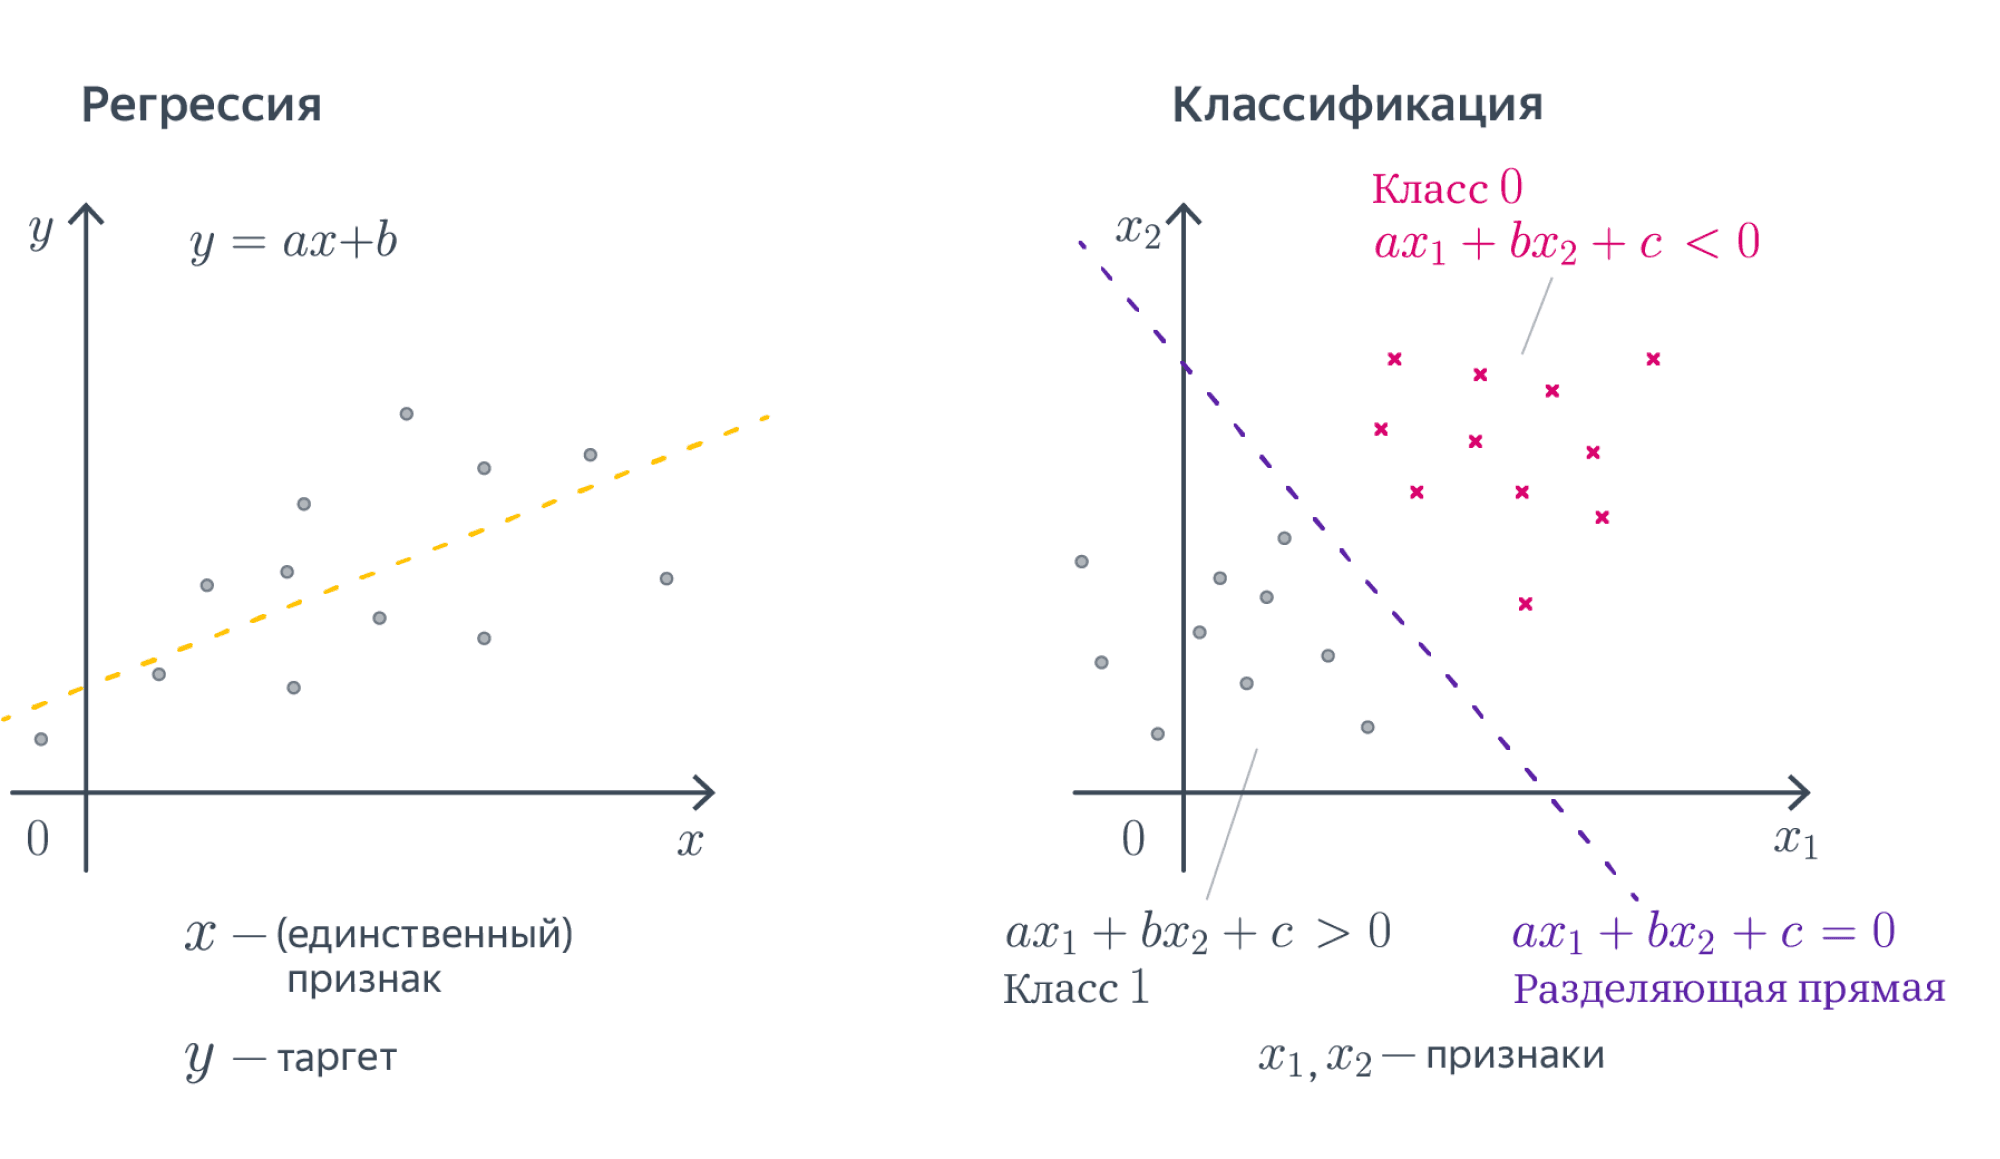
\includegraphics[width=0.11\textwidth]{pics/t_osn24_linear_models.png}
% \end{wrapfigure}

\textbf{Метод наименьших квадратов (МНК)} \\
Пусть у нас задан датасет $(X, y)$, где 
$y=(y_i)_{i=1}^N \in \mathbb{R}^{N}$ – вектор значений целевой переменной, а $X=(x_i)_{i=1}^N \in \mathbb{R}^{N+D}, x_i \in \mathbb{R}^{N}$– матрица объекты-признаки, в которой 
$i$-я строка – это вектор признаков 
$i$-го объекта выборки. Мы хотим моделировать зависимость $y_i$ от $x_i$ как линейную функцию со свободным членом. Общий вид такой функции из $\mathbb{R}^D$ в $\mathbb{R}$ выглядит следующим образом: $ f_{\omega}(x_i)=\langle\omega,x_i\rangle+\omega_0$.
Свободный член $\omega_0$ часто опускают, потому что такого же результата можно добиться, добавив ко всем $x_i$ признак, тождественно равный единице. Будем считать, что это уже сделано и зависимость имеет вид просто $f_\omega(x_i)=\langle\omega,x_i\rangle$. \\
\textbf{Сведение к задаче оптимизации} Мы должны научиться измерять качество модели и минимизировать её ошибку, как-то меняя обучаемые параметры ($\omega$). Функция, оценивающая то, как часто модель ошибается, называется функцией потерь, функционалом качества или лоссом.

Нужно взять вектор $y$ и вектор предсказаний модели и как-то сравнить, насколько они похожи. Расстояние между ними вполне может быть функцией потерь. Положительная непрерывная функция от этого расстояния тоже подойдёт в качестве функции потерь. Возьмем в качестве лосса квадрат $L_2$-нормы вектора разницы предсказаний модели и $y$. $L_2$ - норма разницы – это евклидово расстояние между вектором таргетов и вектором ответов модели, то есть мы их приближаем просто в смысле расстояния.
Так вот, наша функция потерь выглядит так:
\begin{equation*}
    L(f,X,y)=\frac{1}{N}|y-f(X)|_2^2=\frac{1}{N}||y-X\omega||_2^2 =\frac{1}{N}\sum_{i=1}^{N} (y_i-\langle x_i,\omega\rangle)^2
\end{equation*}
Такая функция потерь называется \textbf{Mean Squared Error, MSE или среднеквадратическим отклонением}. \\
Для того чтобы найти лучшую модель, этот функционал нам надо минимизировать по $\omega$: $|y-X\omega|_2^2 \xrightarrow{} \min_{\omega}$

Эту задачу можно решить как аналитически, так и приближенно (например градиентным спуском).
Для точного решения необходимо обратить матрицу $X^TX$, а она может быть вырождена или плохо обусловлена из-за приближенной линейной зависимости признаков. \\
\textbf{Регуляризация} \\
Не всегда решение задачи регрессии единственно. Если в выборке два признака будут линейно зависимы (и следовательно, ранг матрицы будет меньше $D$), то гарантировано найдётся такой вектор весов $\nu$, что $\langle\nu,x_i\rangle=0  
 $ $\forall x_i$. В этом случае, если $\omega$ является решением, то и $\omega+\alpha\nu$ тоже решение для $\forall$ $\alpha$. То есть решение не только не обязано быть уникальным, так ещё может быть сколь угодно большим по модулю. Это создаёт вычислительные трудности. Малые погрешности признаков сильно возрастают при предсказании ответа, а в градиентном спуске накапливается погрешность из-за операций со слишком большими числами. В жизни признаки обычно приближённо линейно зависимыми. Такая ситуация называется \textbf{мультиколлинеарностью}. В этом случае у нас, всё равно, возникают проблемы, близкие к описанным выше. 
\par Для того, чтобы справиться с этой проблемой, задачу обычно \textbf{регуляризуют}, то есть добавляют к ней дополнительное ограничение на вектор весов. Это ограничение можно, как и исходный лосс, задавать по-разному, но, как правило, ничего сложнее, чем $L_1$ (или \textbf{Лассо регуляризация}) и $L_2$ (или \textbf{гребневая регрессия}) - нормы, не требуется. \\
Модифицированная задача: $\min_{\omega}L(f, X, y) = \min_{\omega}(|X\omega-y|_2^2+\lambda|w|_k^k)$. \\
$\lambda$ - это очередной параметр, a $|\omega|_k^k$ - это один из двух вариантов:
$|\omega|_2^2=\omega_1^2+...+\omega_D^2$ или $ |\omega|_1^1=|\omega_1|+...+|\omega_D|$.
Добавка $\lambda|w|_k^k$ называется \textbf{регуляризационным членом} или \textbf{регуляризатором}, а число $\lambda$ – \textbf{коэффициентом регуляризации}.

\textbf{Линейная классификация} Рассмотрим бинарную классификацию, её легко обобщить до задачи классификации на $K$ классов. Пусть теперь таргеты $y$ кодируют принадлежность к множеству -1 и 1, а $x$ - по-прежнему векторы из $\mathbb{R}^D$. Мы хотим обучить линейную модель так, чтобы плоскость, которую она задаёт, как можно лучше отделяла объекты одного класса от другого.
% \begin{wrapfigure}{l}{0.1\textwidth}
%     \centering
%     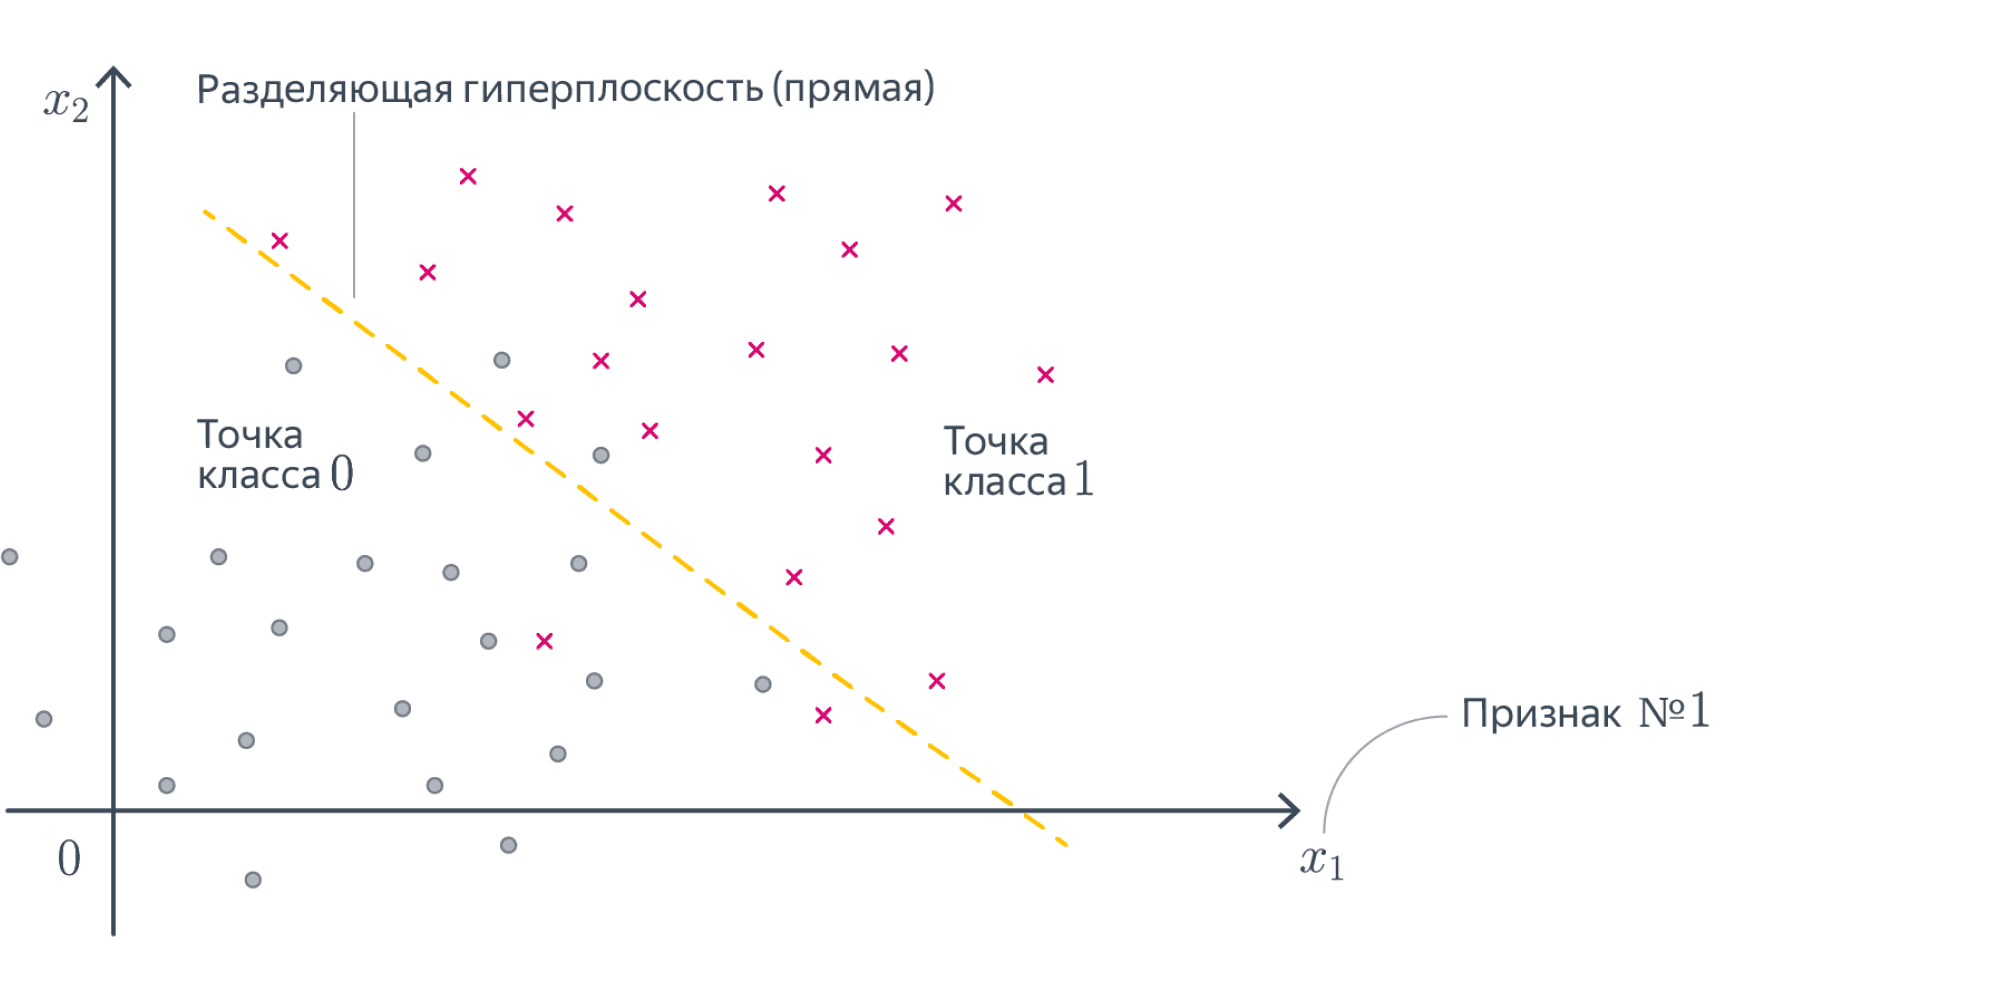
\includegraphics[width=0.1\textwidth]{pics/t_osn24_3.png}
%     %\qquad
%     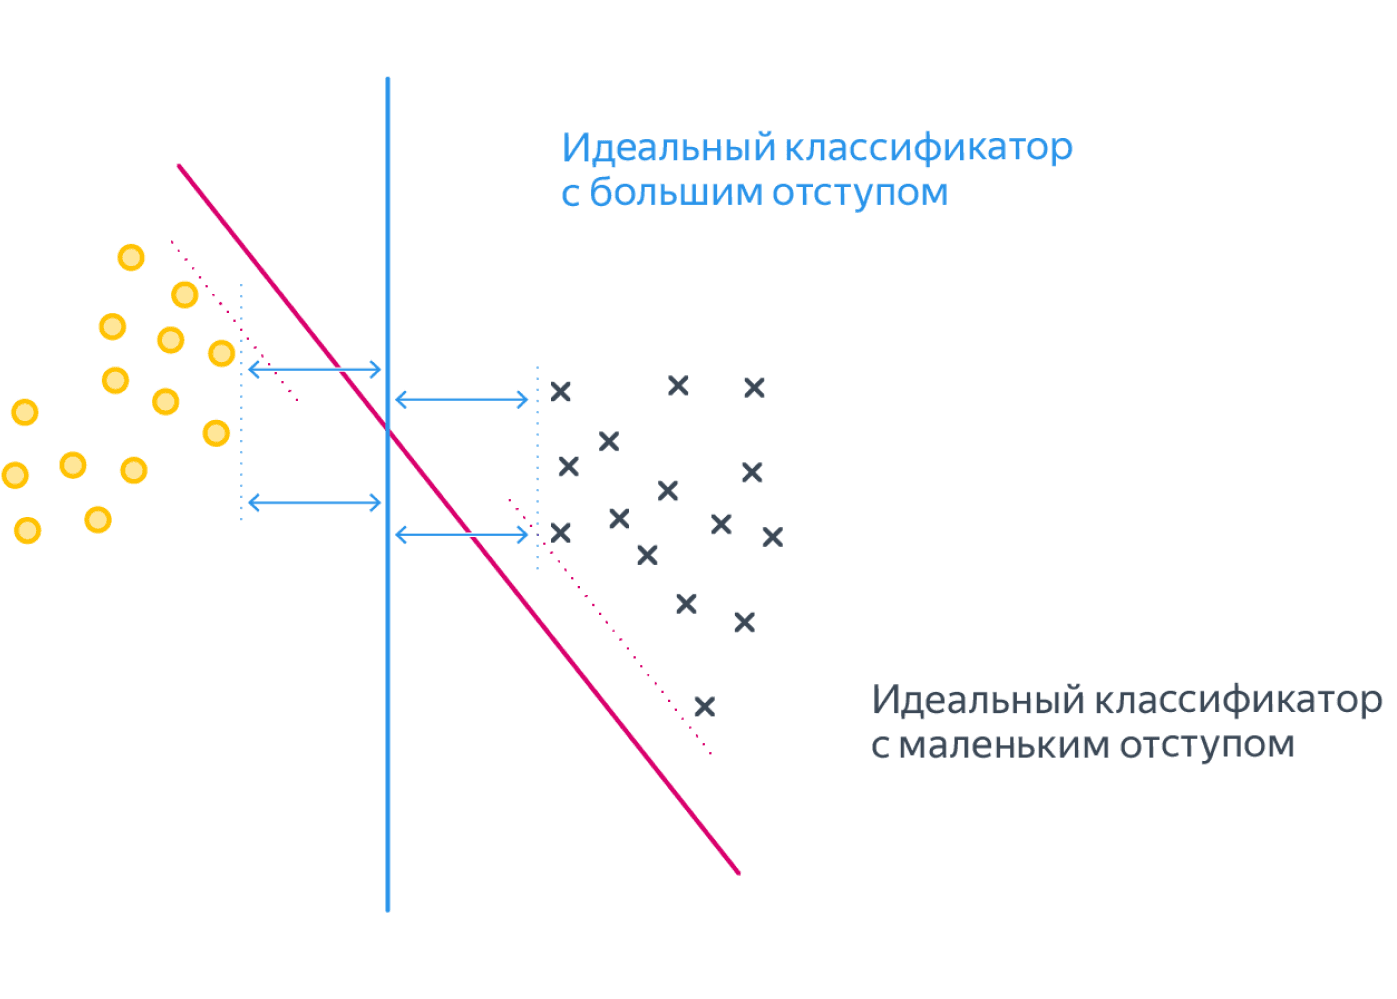
\includegraphics[width=0.1\textwidth]{pics/t_osn24_4.png}
% \end{wrapfigure}

В идеальной ситуации найдётся плоскость, которая разделит классы: положительный окажется с одной стороны от неё, а отрицательный с другой. Выборка, для которой это возможно, называется линейно разделимой. \\
Итоговое предсказание можно будет вычислить по формуле $y = sign\langle\omega,x\rangle$

Сконструируем теперь функционал ошибки. Мы хотим минимизировать число ошибок классификатора, то есть $\sum_i \mathbb{I}[y_i \neq sign \langle w, x_i\rangle]\longrightarrow \min_w$. Домножим обе части на $y_i$ и немного упростим $\sum_i \mathbb{I}[y_i \langle w, x_i\rangle < 0]\longrightarrow \min_w$. Величина $M = y_i \langle w, x_i\rangle$ называется \textbf{отступом} (margin) классификатора. Такая функция потерь называется \textbf{misclassification loss}. Легко видеть, что отступ положителен, когда $sign(y_i) = sign(\langle w, x_i\rangle)$, то есть класс угадан верно; при этом чем больше отступ, тем больше расстояние от $x_i$ до разделяющей гиперплоскости, то есть «уверенность классификатора»; отступ отрицателен, когда $sign(y_i) \ne sign(\langle w, x_i\rangle)$, то есть класс угадан неверно; при этом чем больше по модулю отступ, тем более сокрушительно ошибается классификатор. От каждого из отступов мы вычисляем функцию $F(M) = \mathbb{I}[M < 0] = \begin{cases}1,\ M < 0,\\ 0,\ M\geqslant 0\end{cases}$. Она кусочно-постоянная, и из-за этого всю сумму невозможно оптимизировать градиентными методами: ведь её производная равна нулю во всех точках, где она существует. Но мы можем мажорировать её какой-нибудь более гладкой функцией, и тогда задачу можно будет решить.  \\

\textbf{Hinge loss, SVM} Надо не только найти разделяющую прямую, но и постараться провести её на одинаковом удалении от обоих классов, то есть максимизировать минимальный отступ.
Это можно сделать, поменяв функцию ошибки, а именно положив её равной:
$F(M) = \max(0, 1-M)$.
$$L(w, x, y) = \lambda||w||^2_2 + \sum_i \max(0, 1-y_i \langle w, x_i\rangle)$$
$$\nabla_w L(w, x, y) = 2 \lambda w + \sum_i
        \begin{cases} 
             0,      & \quad      1 - y_i \langle w, x_i \rangle \leq 0 \\ 
            - y_i x_i, & \quad   1 - y_i \langle w, x_i \rangle > 0
        \end{cases}$$ 
Почему же добавленная единичка приводит к желаемому результату? \\ Интуитивно это можно объяснить так: объекты, которые проклассифицированы правильно, но не очень "уверенно" (то есть $0 \leq y_i \langle w, x_i\rangle < 1$), продолжают вносить свой вклад в градиент и пытаются "отодвинуть" от себя разделяющую плоскость как можно дальше. \\
Иначе рассмотреть вопрос поможет вот эта картинка:

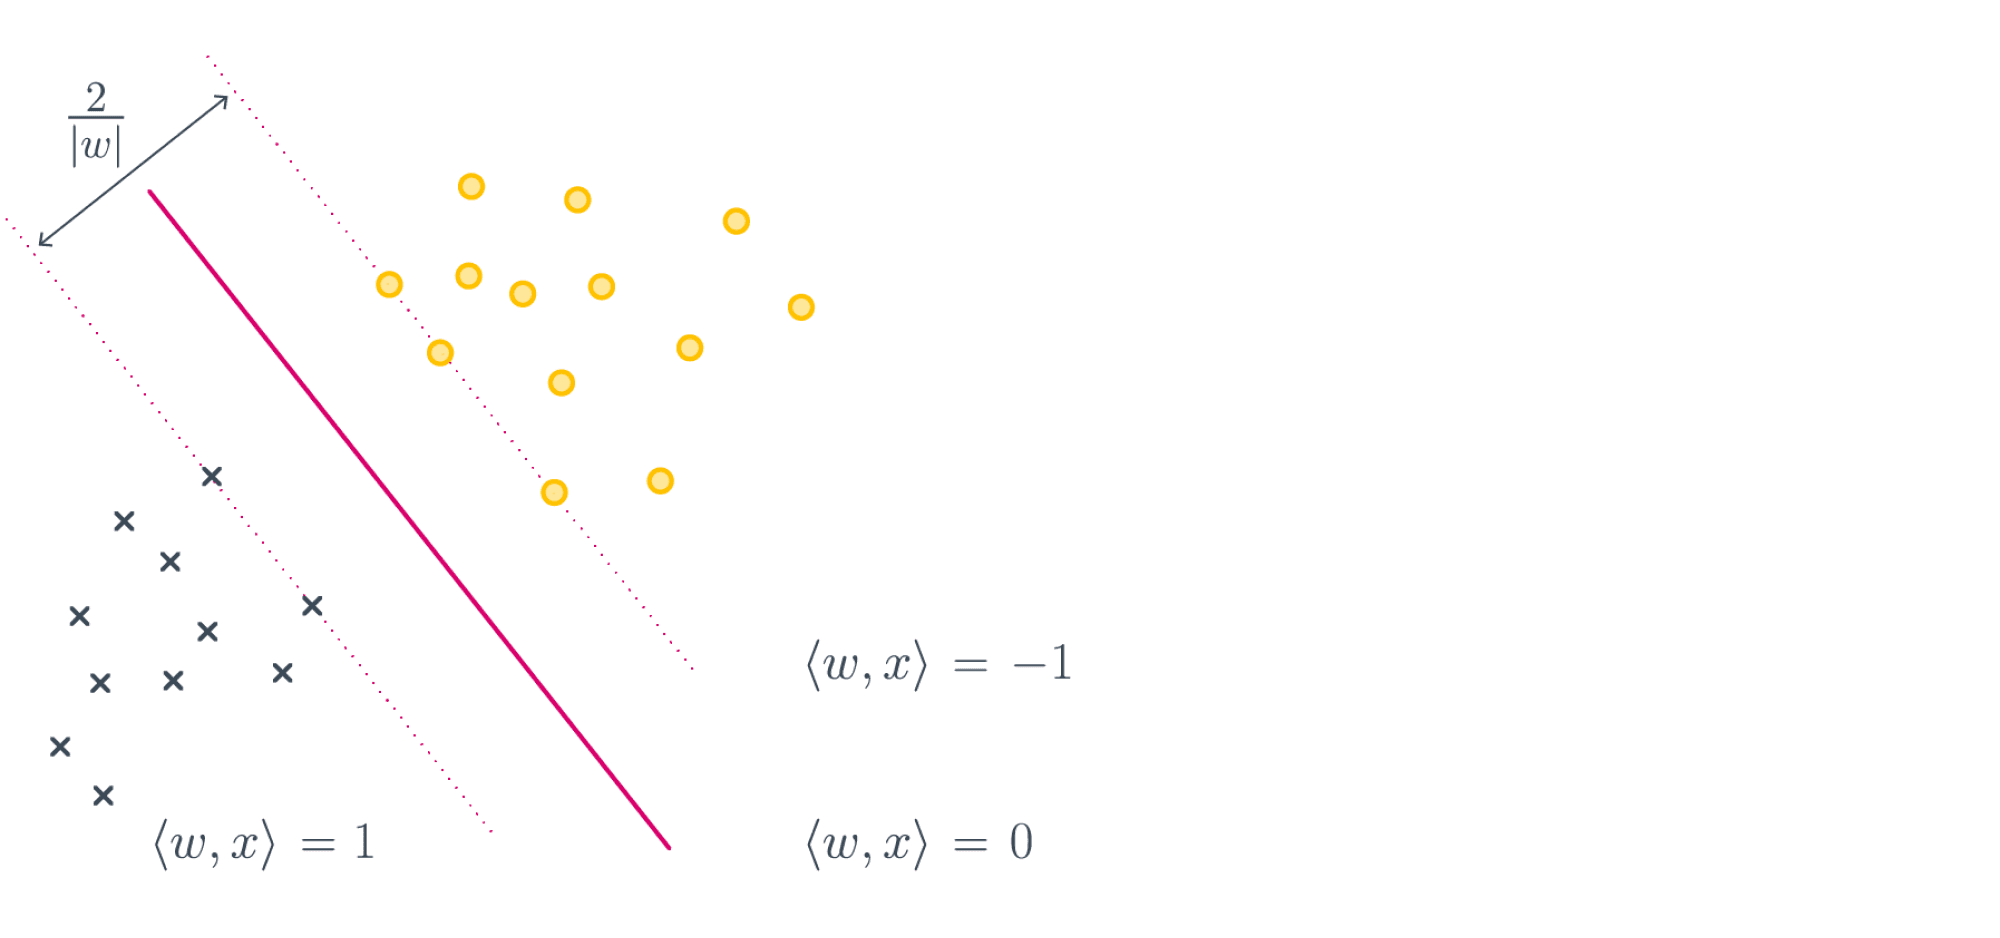
\includegraphics[width=0.15\textwidth]{pics/t_osn24_5.png}


Если мы максимизируем минимальный отступ, то надо максимизировать $\frac{2}{|w|_2}$, то есть ширину полосы при условии того, что большинство объектов лежат с правильной стороны, что эквивалентно решению нашей исходной задачи:
$\lambda|w|^2_2 + \sum_i \max(0, 1-y_i \langle w, x_i\rangle) \longrightarrow\min\limits_{w}$.
Отметим, что первое слагаемое у нас обратно пропорционально ширине полосы, но мы и максимизацию заменили на минимизацию, так что тут всё в порядке. Второе слагаемое – это штраф за то, что некоторые объекты неправильно расположены относительно разделительной полосы, так как классы могут быть линейно неразделимы. \\
Ближайшие к плоскости правильно классифицированные объекты, которые называют \textbf{опорными векторами}. Весь метод называется методом \textbf{опорных векторов}, или \textbf{support vector machine}. 
% -------- source --------
\bigbreak
[\cite{t_osn24_svm_mlbook}]